\documentclass[12pt,a4paper,twocolumn]{article}

% ===== Paquetes básicos =====
\usepackage[spanish]{babel}      
\usepackage[utf8]{inputenc}      
\usepackage[T1]{fontenc}         
\usepackage{amsmath, amssymb}    
\usepackage{graphicx}            
\usepackage{float}               
\usepackage{siunitx}             
\usepackage{tikz}                
\usepackage{circuitikz}
\usepackage{caption}             
\usepackage{geometry}
\usepackage{stfloats}
\usepackage{mhchem}
\usepackage{booktabs}
\usepackage[hyphens]{url}
\usepackage{hyperref}
\usepackage{subcaption}
\usepackage{physics}
\urlstyle{same}
\geometry{top=2.5cm,bottom=2.5cm,left=2.5cm,right=2.5cm}
\usepackage{tocloft}
% Texto del índice normal, sin negritas en números
\renewcommand{\cftsecfont}{\normalfont}
\renewcommand{\cftsecpagefont}{\normalfont}

\DeclareSIUnit{\calorie}{cal}
\sisetup{
    output-decimal-marker = {,},
    separate-uncertainty = true,  % Esto muestra ± en lugar de ()
    uncertainty-separator = {\,\pm\,}
}

% ===== Estilo de captions =====
\captionsetup[figure]{labelfont=bf}
\captionsetup[table]{labelfont=bf, name=Tabla}

% ===== Palabras clave =====
\newcommand{\keywords}[1]{\vspace{2mm}\noindent\textbf{Palabras clave:} #1}

% ===== Títulos de secciones =====
\usepackage{sectsty}
%\allsectionsfont{\centering\uppercase}
\sectionfont{\centering\normalsize\uppercase}
\subsectionfont{\centering\small\uppercase}
\subsubsectionfont{\centering\small\itshape}
\renewcommand{\thesection}{\Roman{section}}

% ===== Datos del informe (centrado) =====
\title{\textbf{\LARGE Determinación experimental de la relación carga-masa del electrón mediante el método Busch}}
\author{
\large Francisco Utrera - Omar Khalid Daus\\[2mm]
\small \textit{Informe de Experimental II -- Instituto Balseiro} \\
\small \textit{Universidad Nacional de Cuyo \& Comisión Nacional de Energía Atómica} \\
\small \textit{Av. Bustillo 9500, c.p.8400 San Carlos de Bariloche, Río Negro, Argentina} \\
\small \texttt{francisco.utrera@ib.edu.ar} \texttt{omar.daus@ib.edu.ar} %tu mail khalid
}
\date{\today}

\begin{document}

% ===== Portada =====
\twocolumn[
\begin{@twocolumnfalse}
    \maketitle
    \begin{abstract}
    En el presente trabajo se recreó el método de Busch para la determinación de la relación carga-masa del electrón. Dicho
    método consiste en determinar mínimos de área de impacto de electrones en la pantalla de un tubo de rayos catódicos que
    está dentro de un cilindro con un campo magnético homogéneo $B,$ impartiendo distintas tensiones de aceleración $V$ a los
    electrones, a modo de calcular el valor de $e/m$ a partir de la ubicación de los mínimos. 
    El valor determinado experimentalmente resultó ser $e/m=\left( 6,7 \pm 0,4 \right)\times 10^{11}\,\unit{\coulomb\per\kilogram}.$
    Se observaron numerosas dificultades en la recreación del método de Busch que fueron cruciales para la inconsistencia de lo obtenido con lo tabulado: 
    la principal de ellas, una mala calibración del campo magnético, de modo que no era uniforme y su valor calculado se cree distinto al real. 
    A pesar de estas limitaciones, el resultado obtenido es satisfactorio en tanto se alcanzó a conocer la relación en orden de magnitud que tienen la carga y la masa del electrón ($10^{11}\,\unit{\coulomb\per\kilogram}$).
    \end{abstract}
    \keywords{método Busch, campo magnético, relación carga-masa del electrón}
    \vspace{1cm}
\end{@twocolumnfalse}
]


% ===== Secciones =====

\section{Introducción}
En el año 1922, Hans Busch presenta teóricamente que cualquier campo magnético o eléctrico de simetría axial es capaz de enfocar un haz de electrones de forma análoga a la que una lente actúa sobre un haz de luz. Tal aporte da inicio así a la óptica electrónica y fue crucial para la invención del microscopio electrónico en 1931. Posteriormente, en el año 1926, y con bases en su aporte teórico previo, Busch propone y detalla un método preciso para la determinación de la relación carga-masa del electrón (e/m). 

En el método de Busch se aceleran electrones en un tubo de rayos catódicos y se los somete posteriormente al efecto de un campo magnético colineal con el eje del tubo. Se puede considerar que la fuente de origen de los electrones es puntual y se supone homogeneidad del campo magnético en todo el trayecto de aquellos. A su vez, la diferencia de potencial \textit{V} con la cual se acelera a los electrones se supone lo suficientemente alta para que las componentes de sus velocidades satisfagan que $
|\mathbf{v_\parallel}| \gg |\mathbf{v_\perp}|$ (respecto a la dirección del campo magnético). Tomando la fuerza de Lorentz, se tiene:

\begin{equation}
    \mathbf{F} = e(\mathbf{v_\perp\times\mathbf{B}})\,,
\end{equation}

\noindent donde \textit{e} es la carga del electrón. Se observa que el campo magnético no hace fuerza sobre la componente paralela de la velocidad, por lo cual puede suponerse que se mantiene constante a lo largo de toda la trayectoria. A su vez, debido a que el haz puede no estar perfectamente colimado, las pequeñas componentes transversales de la velocidad son tales que el electrón produce órbitas helicoidales. Se toma, de este modo, la frecuencia angular del movimiento circular que se describe transversalmente al campo magnético:

\begin{equation}
    \omega = |\mathbf{v_\perp}|r\,,
    \label{eq:omega-vperp}
\end{equation}

\noindent donde \textit{r} es el radio del círculo descrito transversalmente a $\mathbf{B}$. Sea ahora un conjunto de electrones que parten desde un fuente puntual. Dado que se supone al campo magnético con simetría axial, las distintas velocidades transversales son tales que respetan una distribución de probabilidad dependiente de la distancia al eje (\textit{r}). Ahora bien, considerando la dinámica circular que describe la componente perpendicular y tomando la Ecuación \ref{eq:omega-vperp}, puede observarse que,

\begin{equation}
    \omega = \frac{e}{m}|\mathbf{B}|\,,
    \label{eq:omega}
\end{equation}

\noindent con \textit{m} la masa del electrón. Dado que los electrones parten desde la misma fuente puntual y tienen la misma velocidad angular, sin importar la velocidad transversal, todos se focalizan en las misma distancias $l_n = nT|\mathbf{v_\parallel}|$, con $n$ un entero y $T$ el período de las órbitas. Considerando entonces la Ecuación \ref{eq:omega},

\begin{equation}
    |\mathbf{v_\parallel}| = \frac{l_n}{2n\pi}\frac{e}{m}|\mathbf{B}|\,,
    \label{eq:vpar}
\end{equation}

\noindent para lo cual se supone además ausencia de fuerzas repulsivas entre los electrones. La Ecuación \ref{eq:vpar} señala que para una dada distancia a la fuente de electrones y a \textit{V} constante, hay distintos órdenes $n$ para los cuales el haz se focaliza en un punto. 

Finalmente, por conservación de energía para la suposición $|\mathbf{v_\parallel}| \gg |\mathbf{v_\perp}|$, se tiene:

\begin{equation}
    |\mathbf{v_\parallel}|^2 = 2\frac{e}{m}V\,,
\end{equation}

\noindent con lo cual, dada la Ecuación \ref{eq:vpar}, se concluye:

\begin{equation}
    V = \frac{l_n^2}{8n^2\pi^2}\frac{e}{m}|\mathbf{B}|^2\,.
    \label{eq:Busch}
\end{equation}

Luego, para un dado \textit{V} en la fuente de electrones, variar $|\mathbf{B}|$ permite desplazar las distancias $l_n$ en las cuales se enfoca el haz. Siendo así, sobre una pantalla a distancia \textit{D} fija de la fuente, se obtiene una distribución del impacto de electrones que se focaliza en un punto cuando $D = l_n$ (a un \textit{n} dado). Cada focalización, o mínimo de la sección transversal del haz, para variaciones de $|\mathbf{B}|$ a un dado \textit{V} se corresponden a distintos órdenes de $n$. Nótese a su vez que estos mínimos son equidistantes en $|\mathbf{B}|$ entre sí dada la periodicidad de las órbitas. Y es a través de estos mínimos que, dada la Ecuación \ref{eq:Busch}, puede hallarse la relación e/m con la proporcionalidad entre \textit{V} y $|\mathbf{B}|^2$.

De este modo, se tiene por objetivo del presente trabajo recrear el método Busch para la determinación de la relación carga-masa del electrón. Se implementará así un tubo de rayos catódicos como fuente emisora de electrones y una pantalla sobre la cual observar la distribución de sus impactos. Variando diferencias de potencial para la aceleración de electrones y el campo magnético en el cual se hallan inmersos, se estudiarán los mínimos de sección transversal en la distribución de sus impactos sobre la pantalla. Son aquellos los que permitirán, en base a la Ecuación \ref{eq:Busch}, obtener la relación e/m, estudiar su apreciación y comparación con valores tabulados y así extraer conclusiones sobre la recreación del método de Busch que será llevado a cabo.


\section{Método experimental}
El experimento comenzó con la calibración del campo magnético $\mathbf{B}.$ Para esto se hizo uso de 5 bobinas, $A_1,\, A_2,\, A_3,\, B_1,\, B_2$,
, cada una con un reóstato en serie. Dichas bobinas se encargan de generar el campo magnético $\mathbf{B}$ dentro del cilindro donde irá el tubo de rayos catódicos. Cabe recalcar que dicho cilindro se encuentra inclinado de forma tal
que su eje es paralelo a la dirección del campo magnético terrestre, de modo que el campo generado por las bobinas se suma directamente con el terrestre.

Se hizo uso de un multímetro Fluke179 True RMS para medir la corriente total $I$ del circuito y una fuente GW Instek PSH-3020A
para suministrar corriente al circuito, como se observa en la Figura \ref{fig:arreglo}. Para la medición del campo magnético se hizo uso de un gaussímetro LakeShore 425 con una sonda Hall axial.

\begin{figure}[h!]
    \centering
    \begin{tikzpicture}[scale=.9]
        % Paths, nodes and wires:
        \draw (5, 5) to[american inductor, l={$A_1$}] (5, 3);
        \draw (6, 5) to[american inductor, l={$A_2$}] (6, 3);
        \draw (7, 5) to[american inductor, l={$A_3$}] (7, 3);
        \draw (8, 5) to[american inductor, l={$B_1$}] (8, 3);
        \draw (9, 5) to[american inductor, l={$B_2$}] (9, 3);
        \draw (5, 3) to[variable american resistor] (5, 1);
        \draw (6, 3) to[variable american resistor] (6, 1);
        \draw (7, 3) to[variable american resistor] (7, 1);
        \draw (8, 3) to[variable american resistor] (8, 1);
        \draw (9, 3) to[variable american resistor] (9, 1);
        \node[shape=rectangle, minimum width=0.465cm, minimum height=0.465cm](N1) at (6.5, 3){} node[anchor=center] at (N1.text){$R_{A2}$};
        \node[shape=rectangle, minimum width=0.465cm, minimum height=0.465cm](N2) at (7.5, 3){} node[anchor=center] at (N2.text){$R_{A3}$};
        \node[shape=rectangle, minimum width=0.465cm, minimum height=0.465cm](N3) at (5.5, 3){} node[anchor=center] at (N3.text){$R_{A1}$};
        \node[shape=rectangle, minimum width=0.465cm, minimum height=0.465cm](N4) at (8.5, 3){} node[anchor=center] at (N4.text){$R_{B1}$};
        \node[shape=rectangle, minimum width=0.465cm, minimum height=0.465cm](N5) at (9.5, 3){} node[anchor=center] at (N5.text){$R_{B2}$};
        \draw (2, 1) to[ammeter] (4, 1);
        \draw (4, 1) -- (9, 1);
        \draw (2, 2.25) to[american current source] (2, 3.75);
        \draw (2, 1) -- (2, 2.25);
        \draw (2, 3.75) -| (2, 5) -- (5, 5);
        \draw (5, 5) -- (9, 5);
        \node[shape=rectangle, minimum width=1.965cm, minimum height=1.465cm] at (3, 4.25){} node[anchor=center, align=center, text width=2cm, inner sep=6pt] at (3.35, 3.25){GW Instek PSH-3020A};
    \end{tikzpicture}
    \caption{Arreglo experimental para la calibración del campo magnético $\mathbf{B}$.}
    \label{fig:arreglo}
\end{figure}

La calibración consistió en medir el campo $B$ en distintas posiciones dentro del tubo,
 con la ayuda de una vara de madera con el sensor Hall ubicado sobre su punta. 
 Dicha vara era introducida dentro del tubo a distintas profundidades y en cada posición
 se registraban los valores de $B$ e $I,$ luego se variaban los valores de los reóstatos a
 modo de minimizar la variación de $B$ a lo largo del tubo. Una vez obtenido un campo uniforme,
  se procedió a medir el valor del campo $B$ en distintas posiciones del cilindro para
  distintos valores de corriente $I,$ a modo de establecer una relación entra la corriente total $I$
  del circuito y el campo $B.$ Para ver los datalles del proceso ver el Anexo A.

Una vez terminada dicha calibración se procedió a ubicar el tubo de rayos catódicos en la zona de menor variación de campo $B$

\section{Resultados}
Se procede a mostrar los valores de campo magnético $B$ obtenidos en distintas posiciones del cilindro para los valores
de resistencia que minimizan la variación de dicho campo en la Figura \ref{fig:variacion_campo}. Se obtuvo una variación del 2,03\% entre $\SI{15,0\pm0,1}{\centi\meter}$ y $\SI{45,0\pm0,1}{\centi\meter},$
la que será la zona de trabajo del tubo.

\begin{figure}[H]
    \centering
    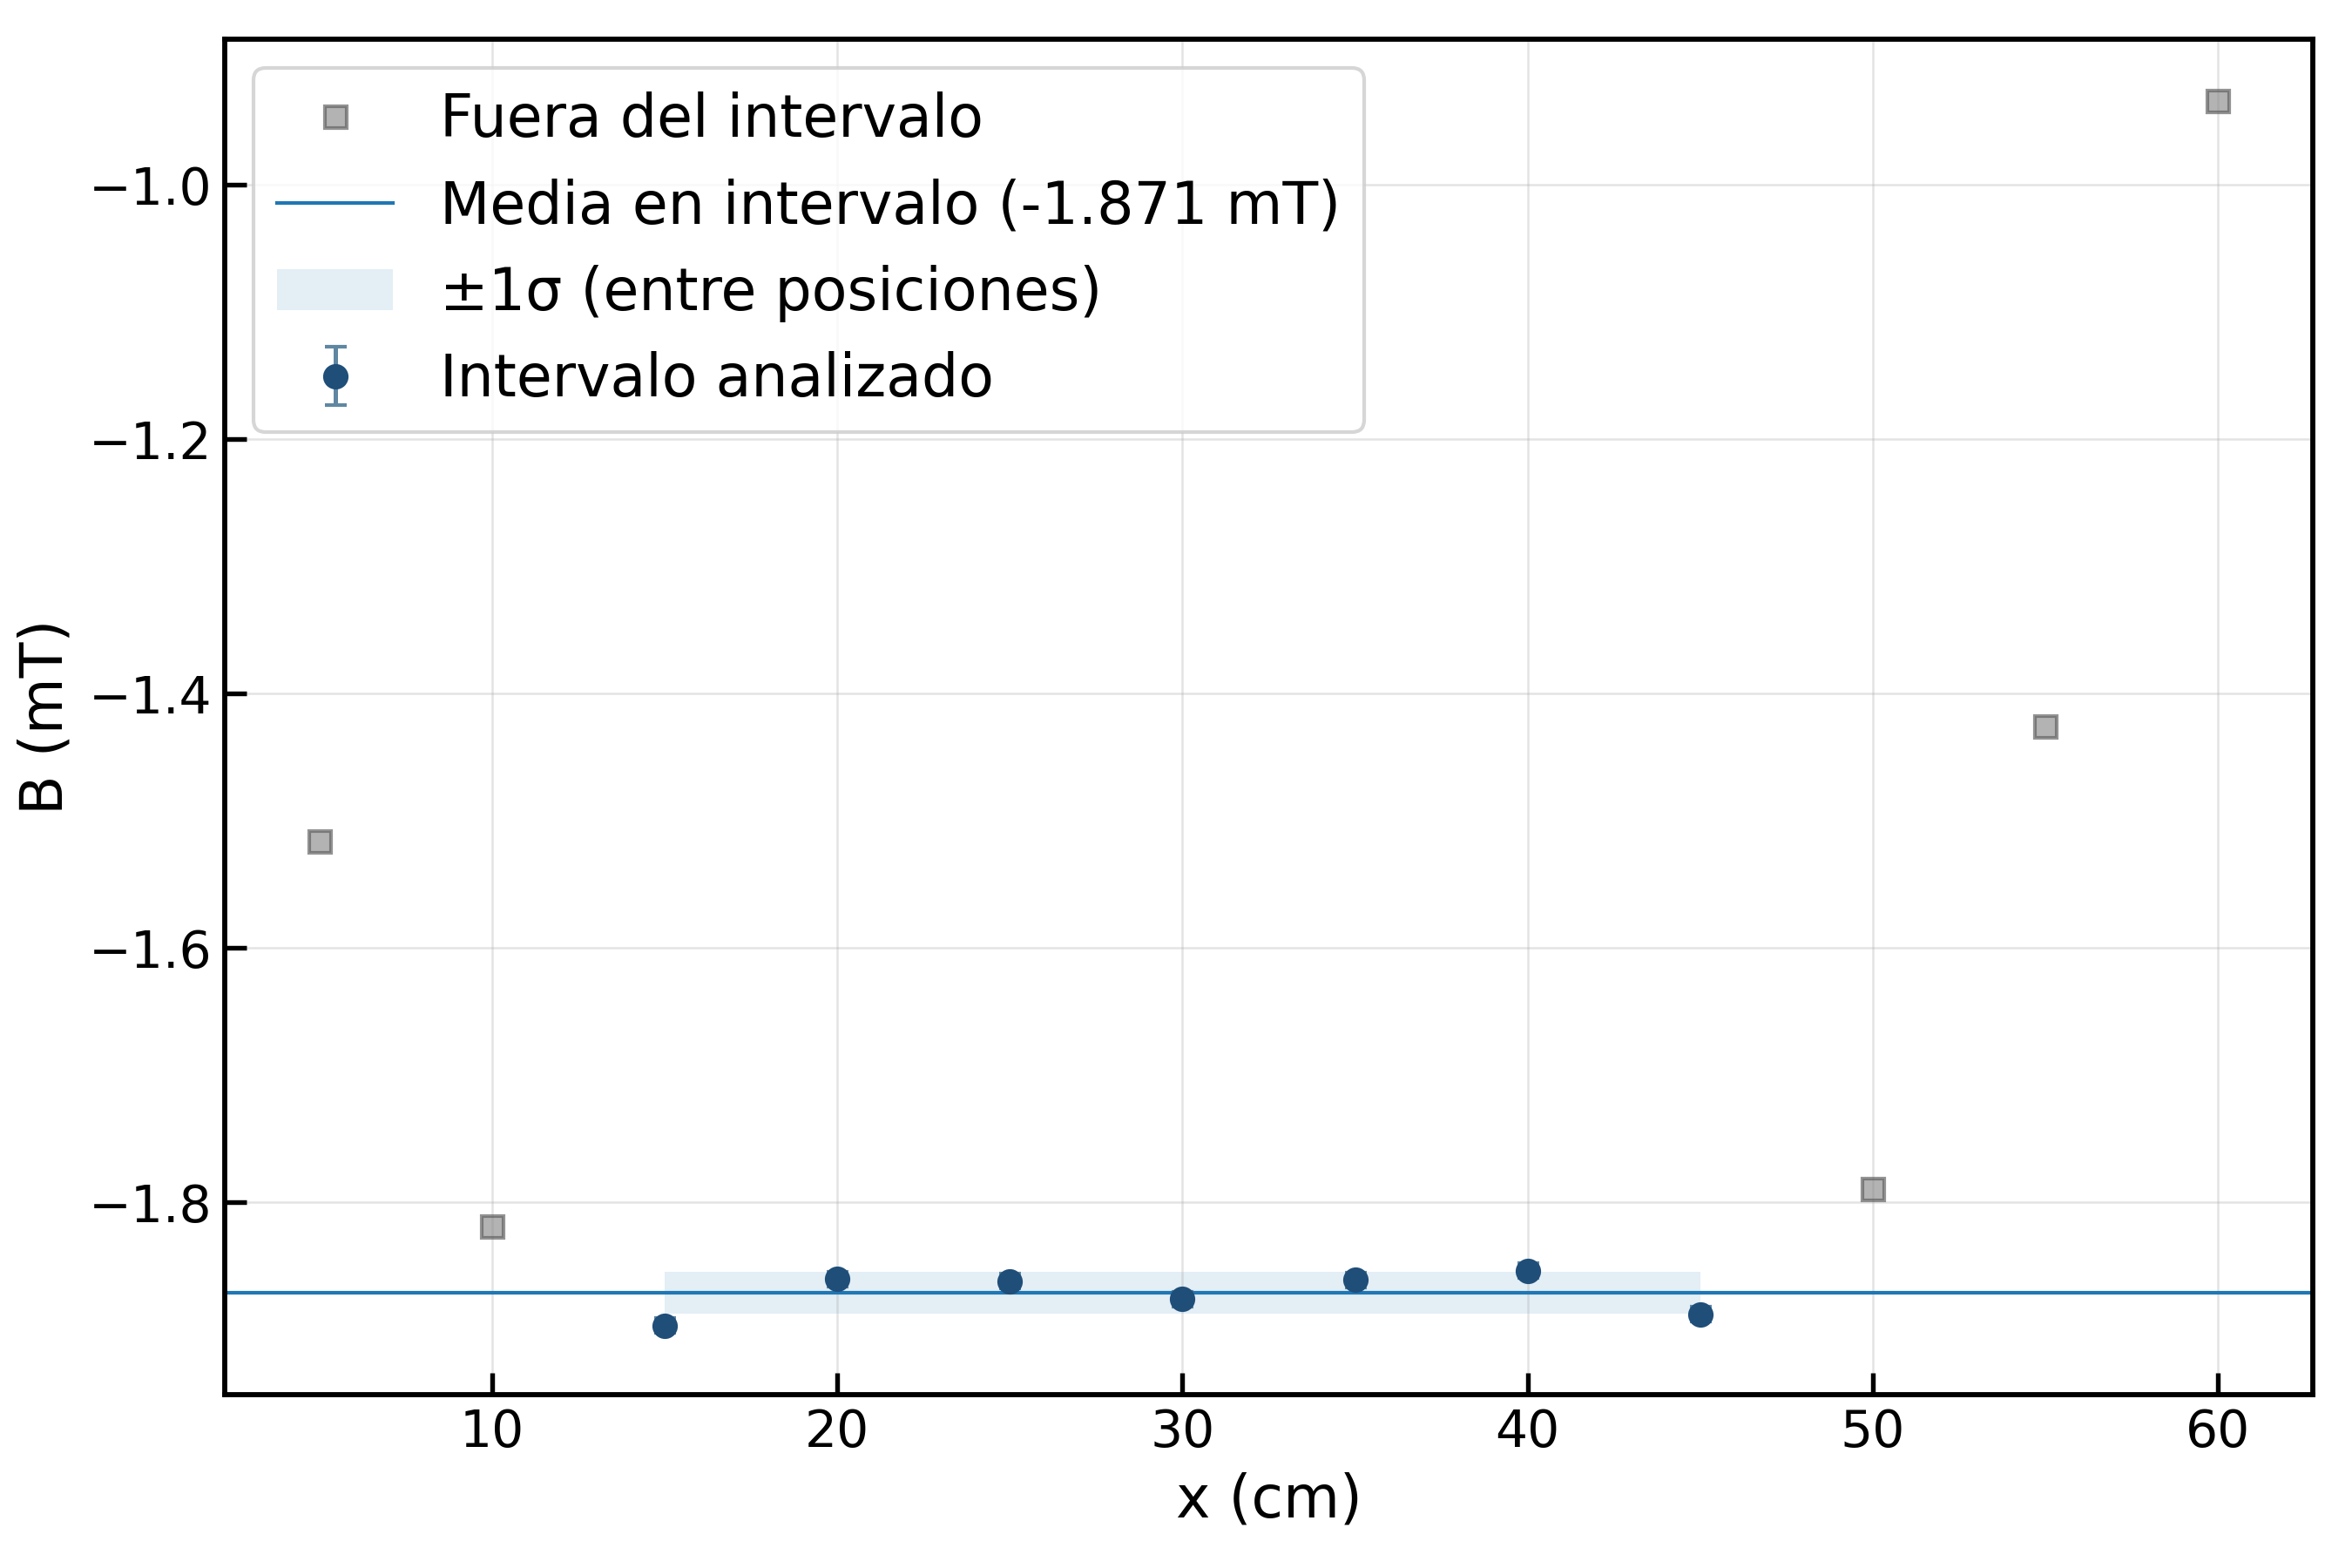
\includegraphics[width=0.49\textwidth]{Images/B_vs_x_mT.png}
    \caption{Campo magnético $B$ en función de la posición $x$ a lo largo del cilindro para $I=\SI{3,00\pm0,03}{\ampere}$.}
    \label{fig:variacion_campo}
\end{figure}

Una vez readaptado el armado experimental, se procedió a encontrar los mínimos relativos de área de impacto de electrones
para distintos valores de tensión de aceleración $V.$ Se muestra en la Figura \ref{fig:area_impacto} como la variación de tensión de alimentación (y por tanto de campo magnético)
afecta al área relativa de impacto para una misma tensión de aceleración.

\begin{figure}[h]
    \centering

    \begin{subfigure}[b]{0.48\columnwidth}
        \centering
        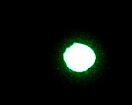
\includegraphics[width=\linewidth]{Images/roi_20260302_162848_V0.016.png}
        \caption{Área de impacto para un bajo valor de $B.$}
        \label{fig:subfig1}
    \end{subfigure}
    \hfill
    \begin{subfigure}[b]{0.48\columnwidth}
        \centering
        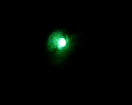
\includegraphics[width=\linewidth]{Images/roi_20260302_163106_V0.062.png}
        \caption{Área de impacto para un alto valor de $B.$}
        \label{fig:subfig2}
    \end{subfigure}

    \caption{Imágenes capturadas por la cámara digital para distintos valores de $B$
    a una tensión de aceleración de $V=\SI{700,00\pm0,05}{\volt}$.}
    \label{fig:area_impacto}
\end{figure}

Para cada valor de tensión de aceleración, se gráfico el área relativa en función de la tensión de alimentación,
a modo de encontrar los mínimos relativos de área relativa. Esto se muestra en la Figura \ref{fig:area_vs_V}.

\begin{figure}[h]
    \centering
    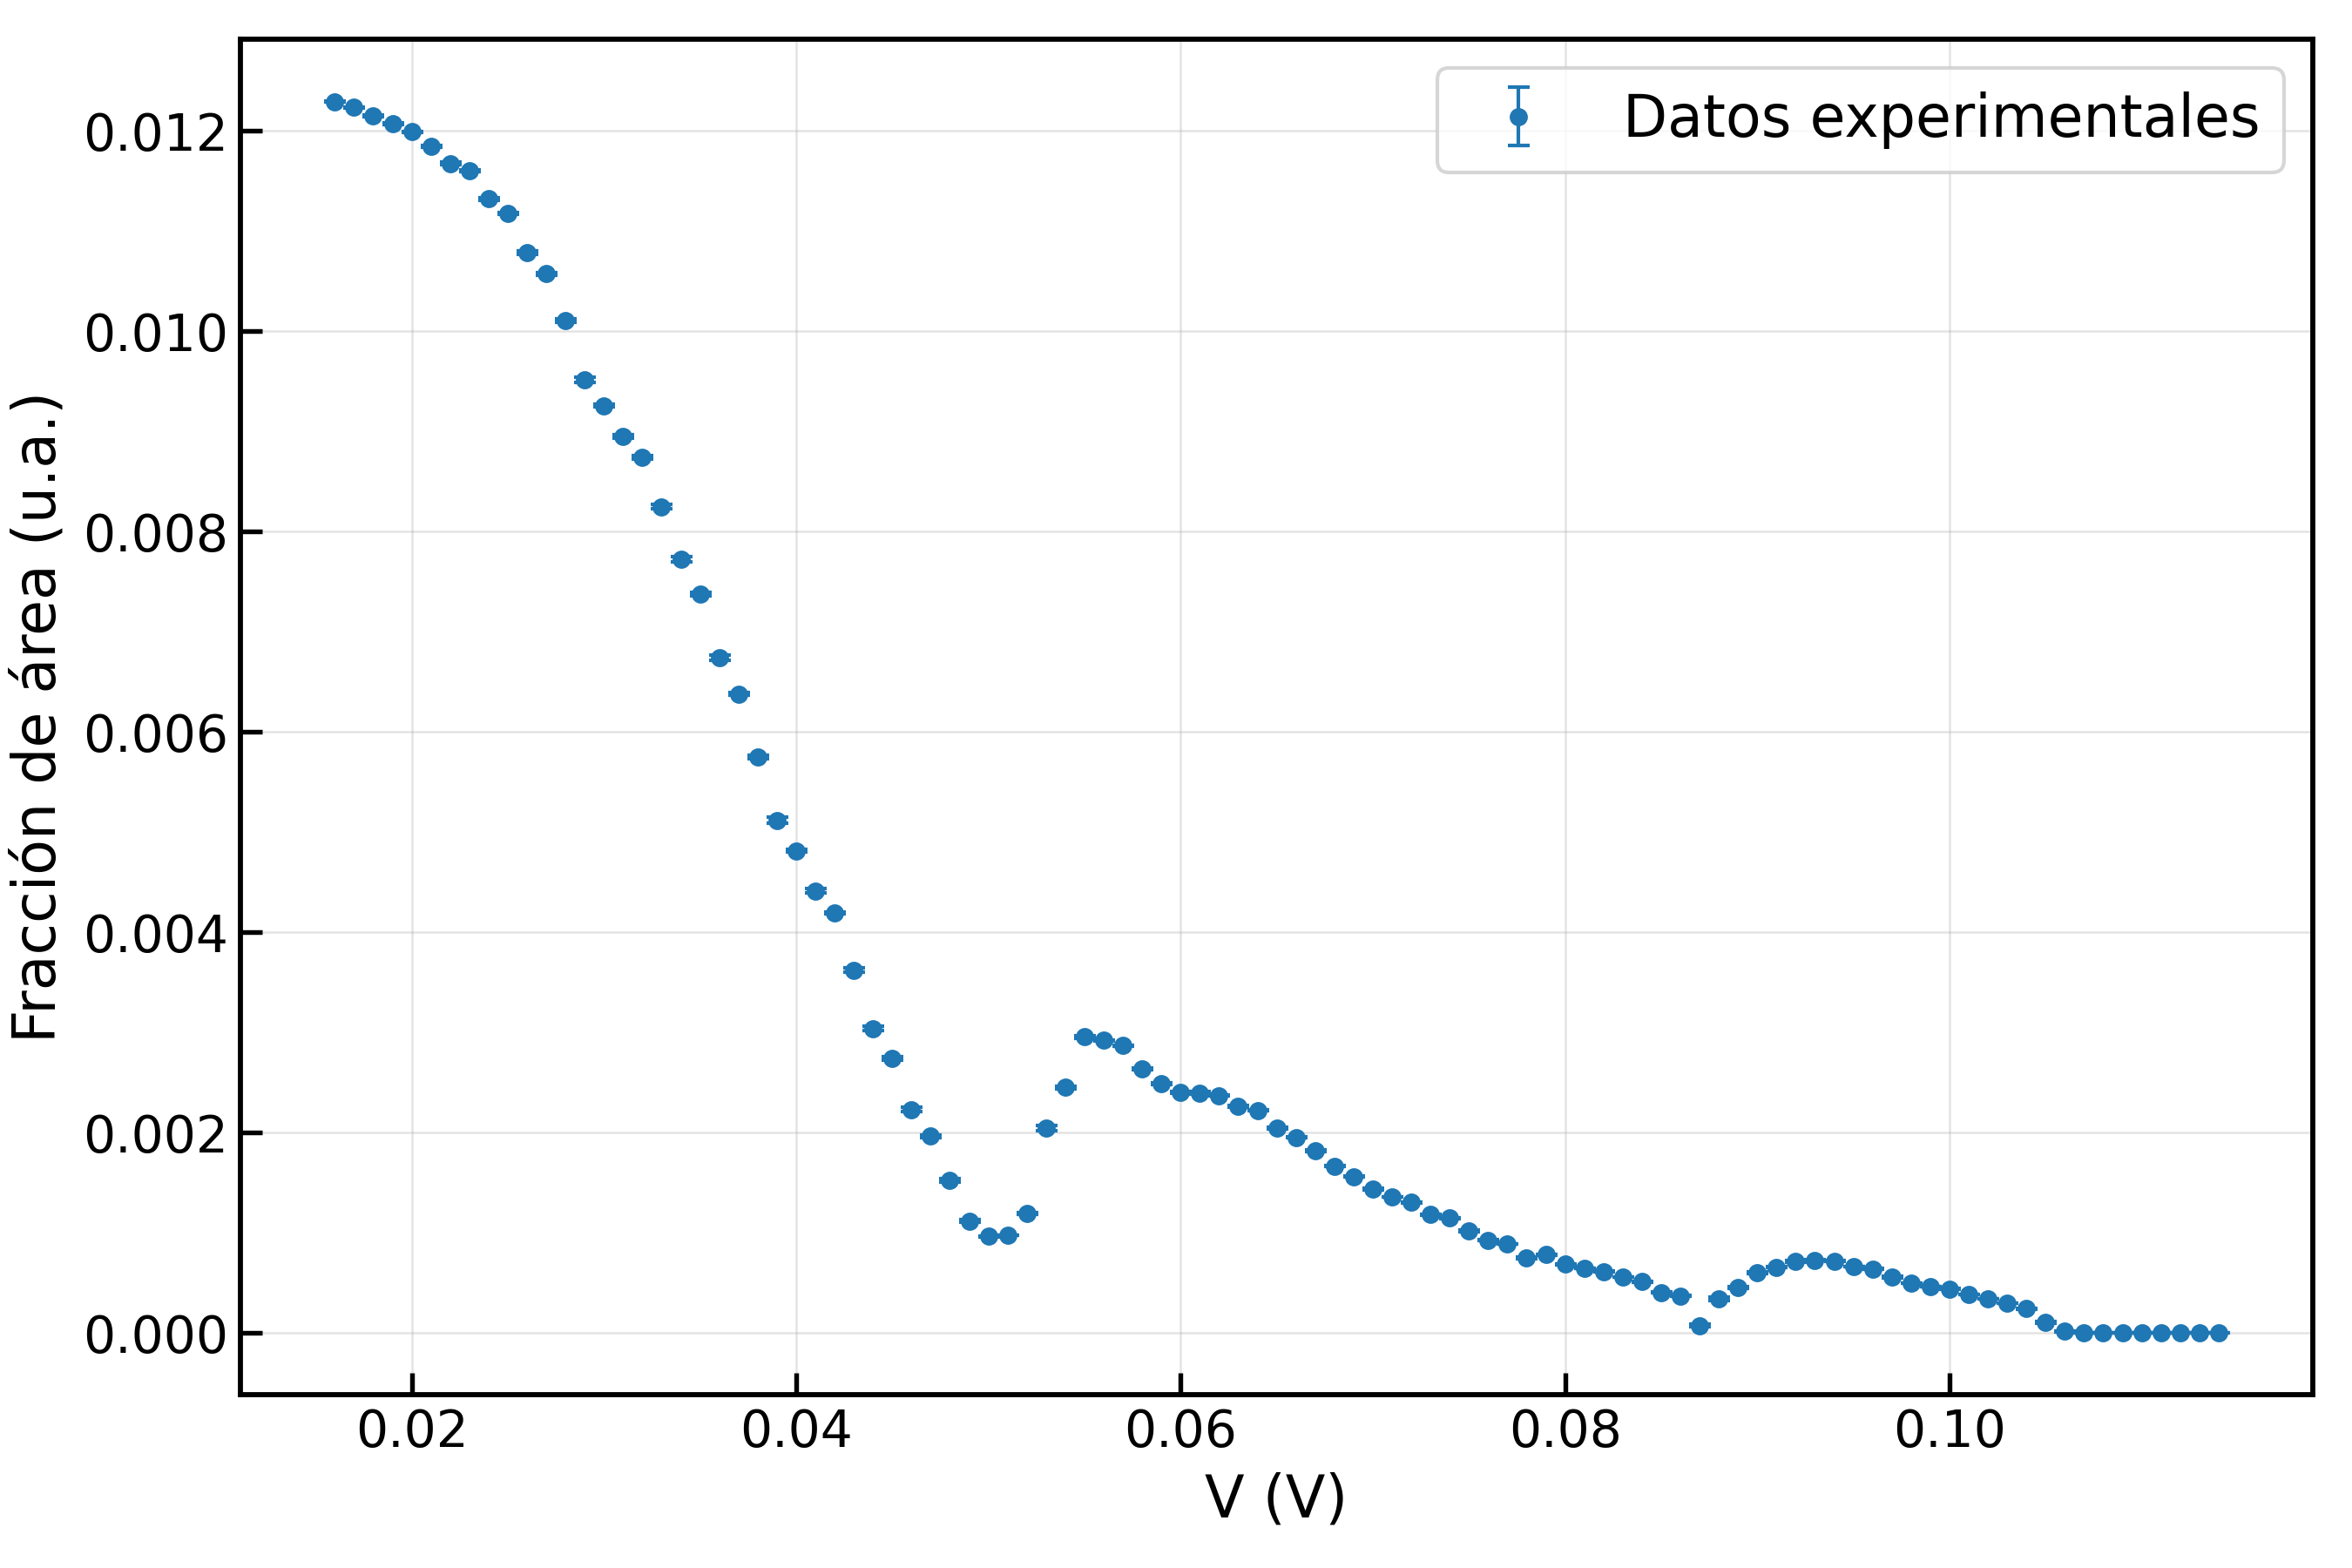
\includegraphics[width=\columnwidth]{Images/frac_vs_V.png}
    \caption{Área relativa de impacto en función de la tensión de alimentación para una tensión de aceleración $V=\SI{500,00\pm0,05}{\volt}$.}
    \label{fig:area_vs_V}
\end{figure}

Se observa una curva similar a la esperada por la Ecuación PONER ECUACION CORRESPONDIENTE, aunque esto no fue así
para otros valores de tensión de aceleración. El por qué de esto se discutirá más adelante.

Luego, mediante un script de Python, se encontraron los mínimos
relativos de área relativa, identificándose además el orden de cada mínimo. Dichos mínimos se muestran en la Figura \ref{fig:minimos}:

\begin{figure}[h]
    \centering
    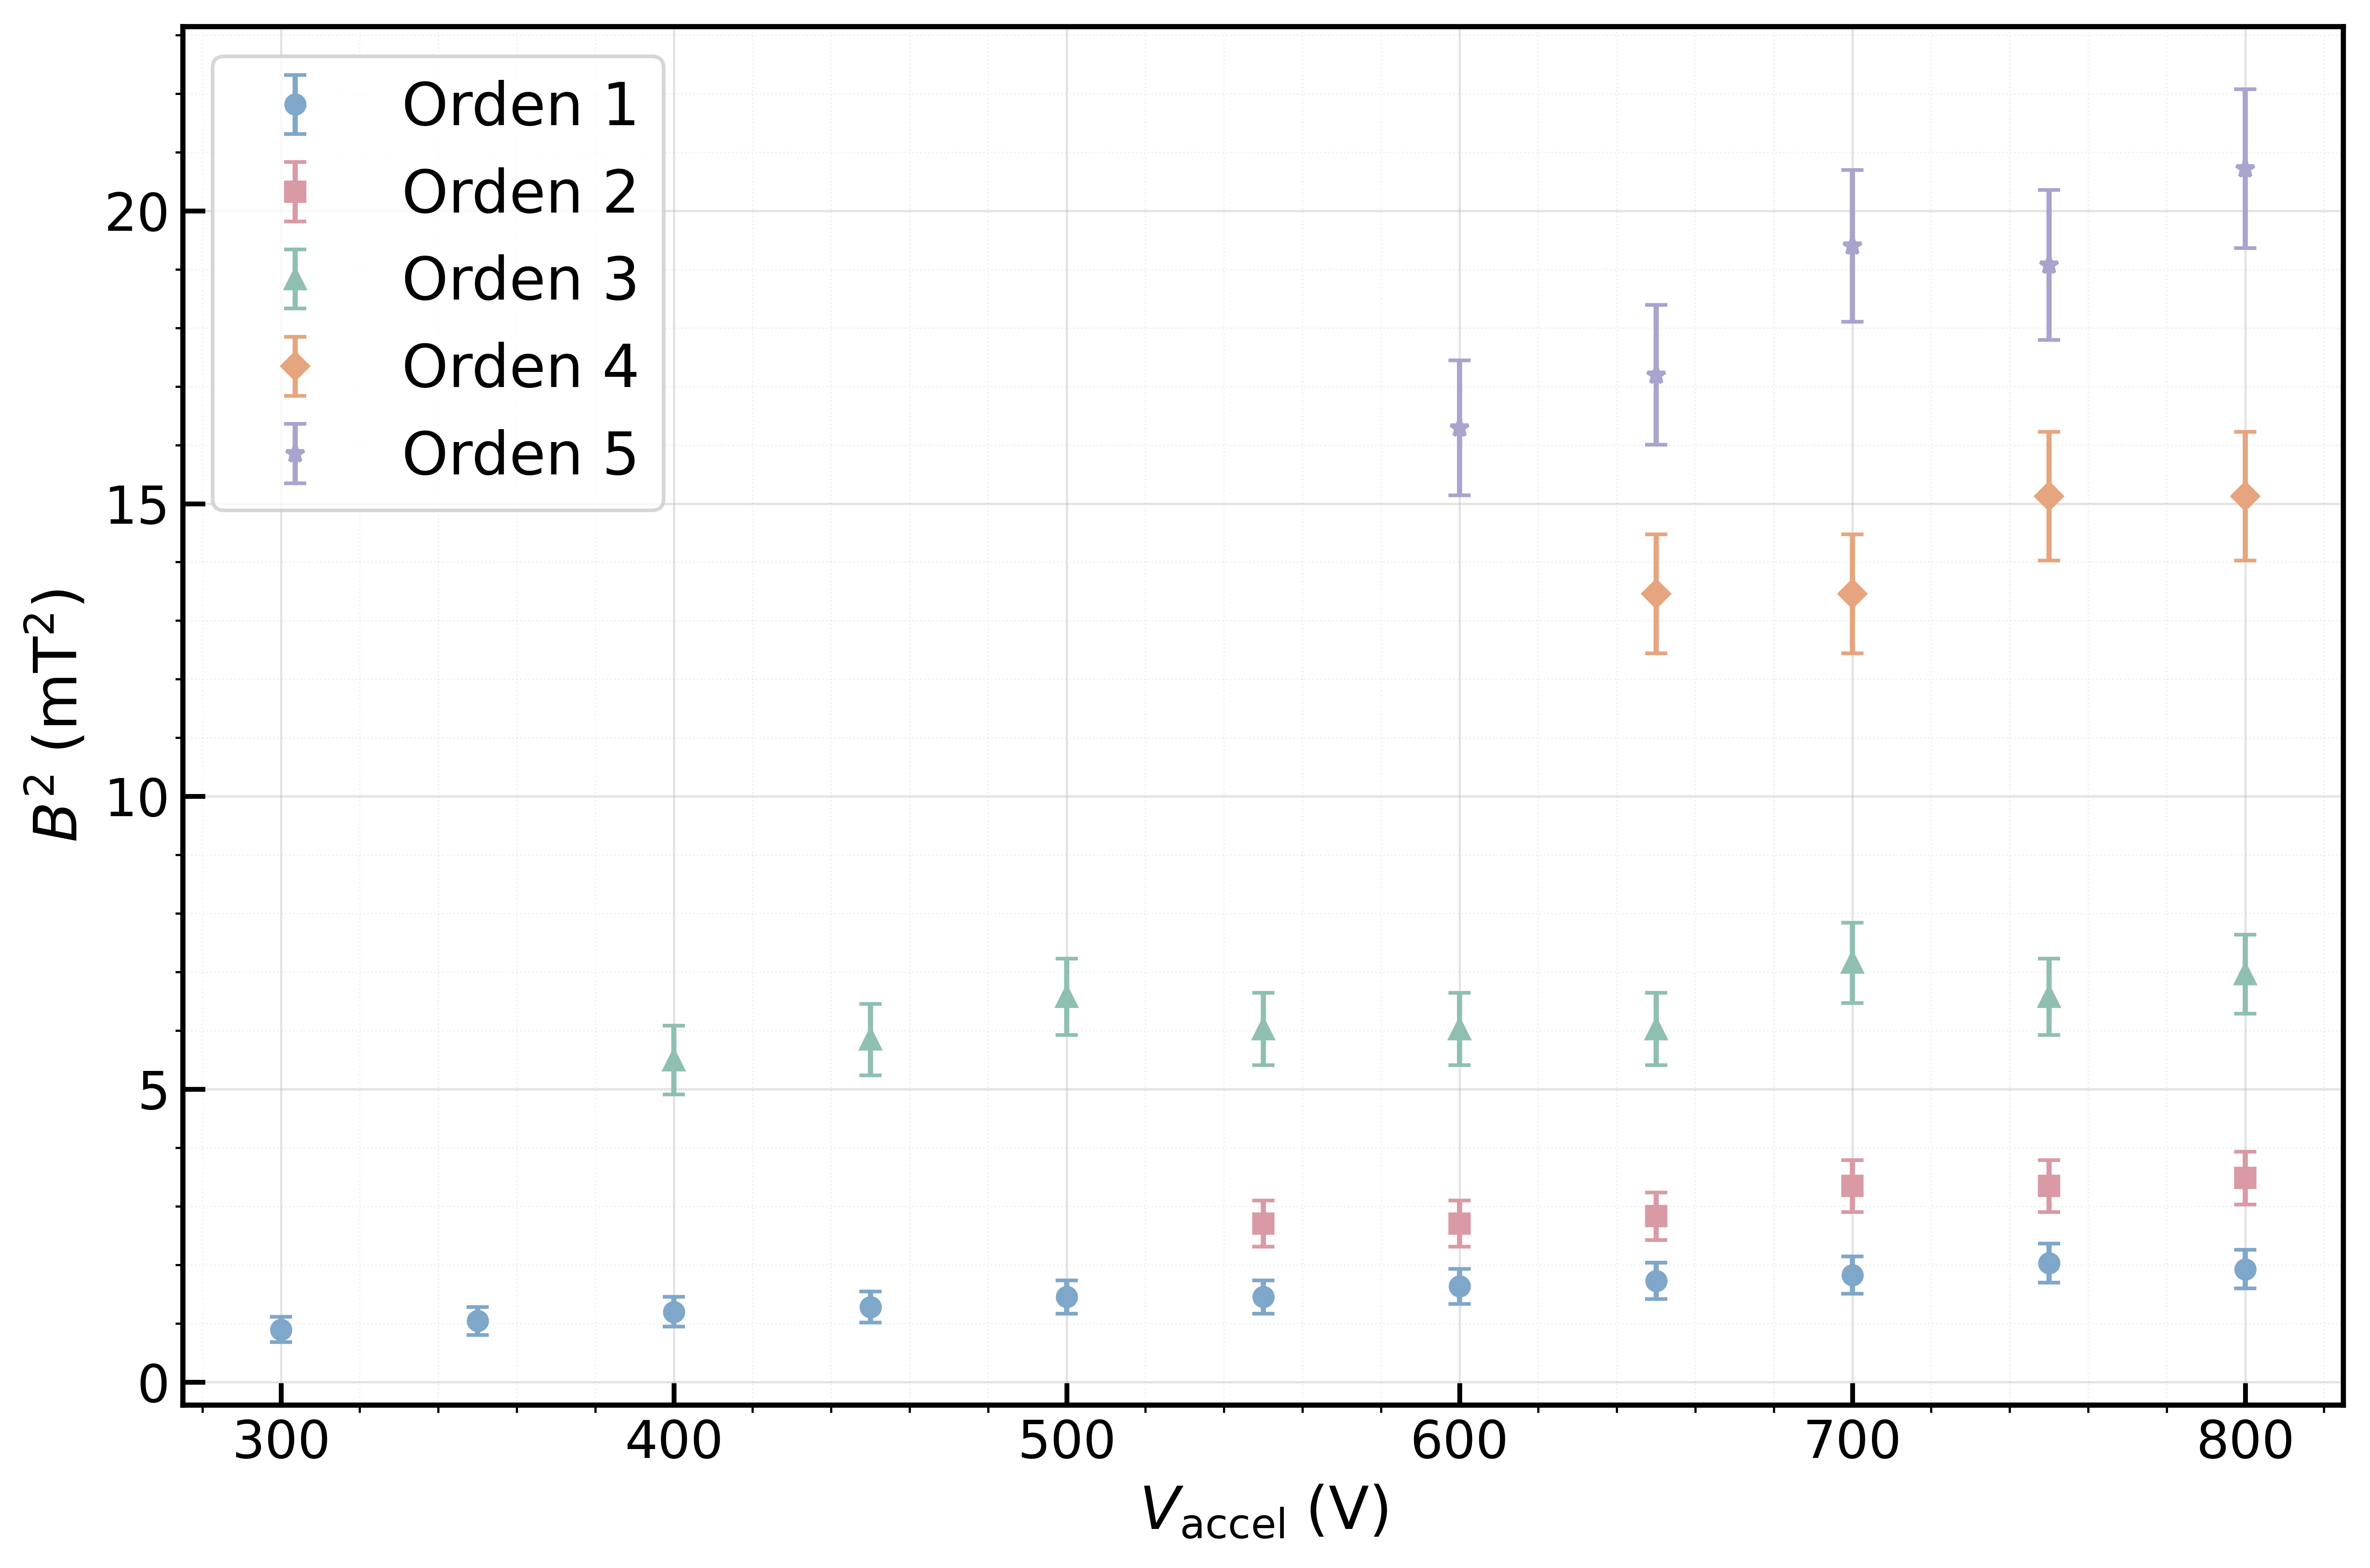
\includegraphics[width=\columnwidth]{Images/Datos BV.png}
    \caption{Valores de campo magnético $B$ que minimizan el área relativa en función de la tensión de aceleración $V.$}
    \label{fig:minimos}
\end{figure}

Para cada orden de mínimos, la relación debería ser lineal, pero se observa que solo algunos ordenes cumplen esto, lo que es inconsistente
con la teoría. Luego se procedió a normalizar por $n^2$, ya que dicha relación debería ser lineal y se realizó un ajuste de dichos datos. Esto se muestra en la Figura \ref{fig:minimos_normalizados}:

\begin{figure}[h]
    \centering
    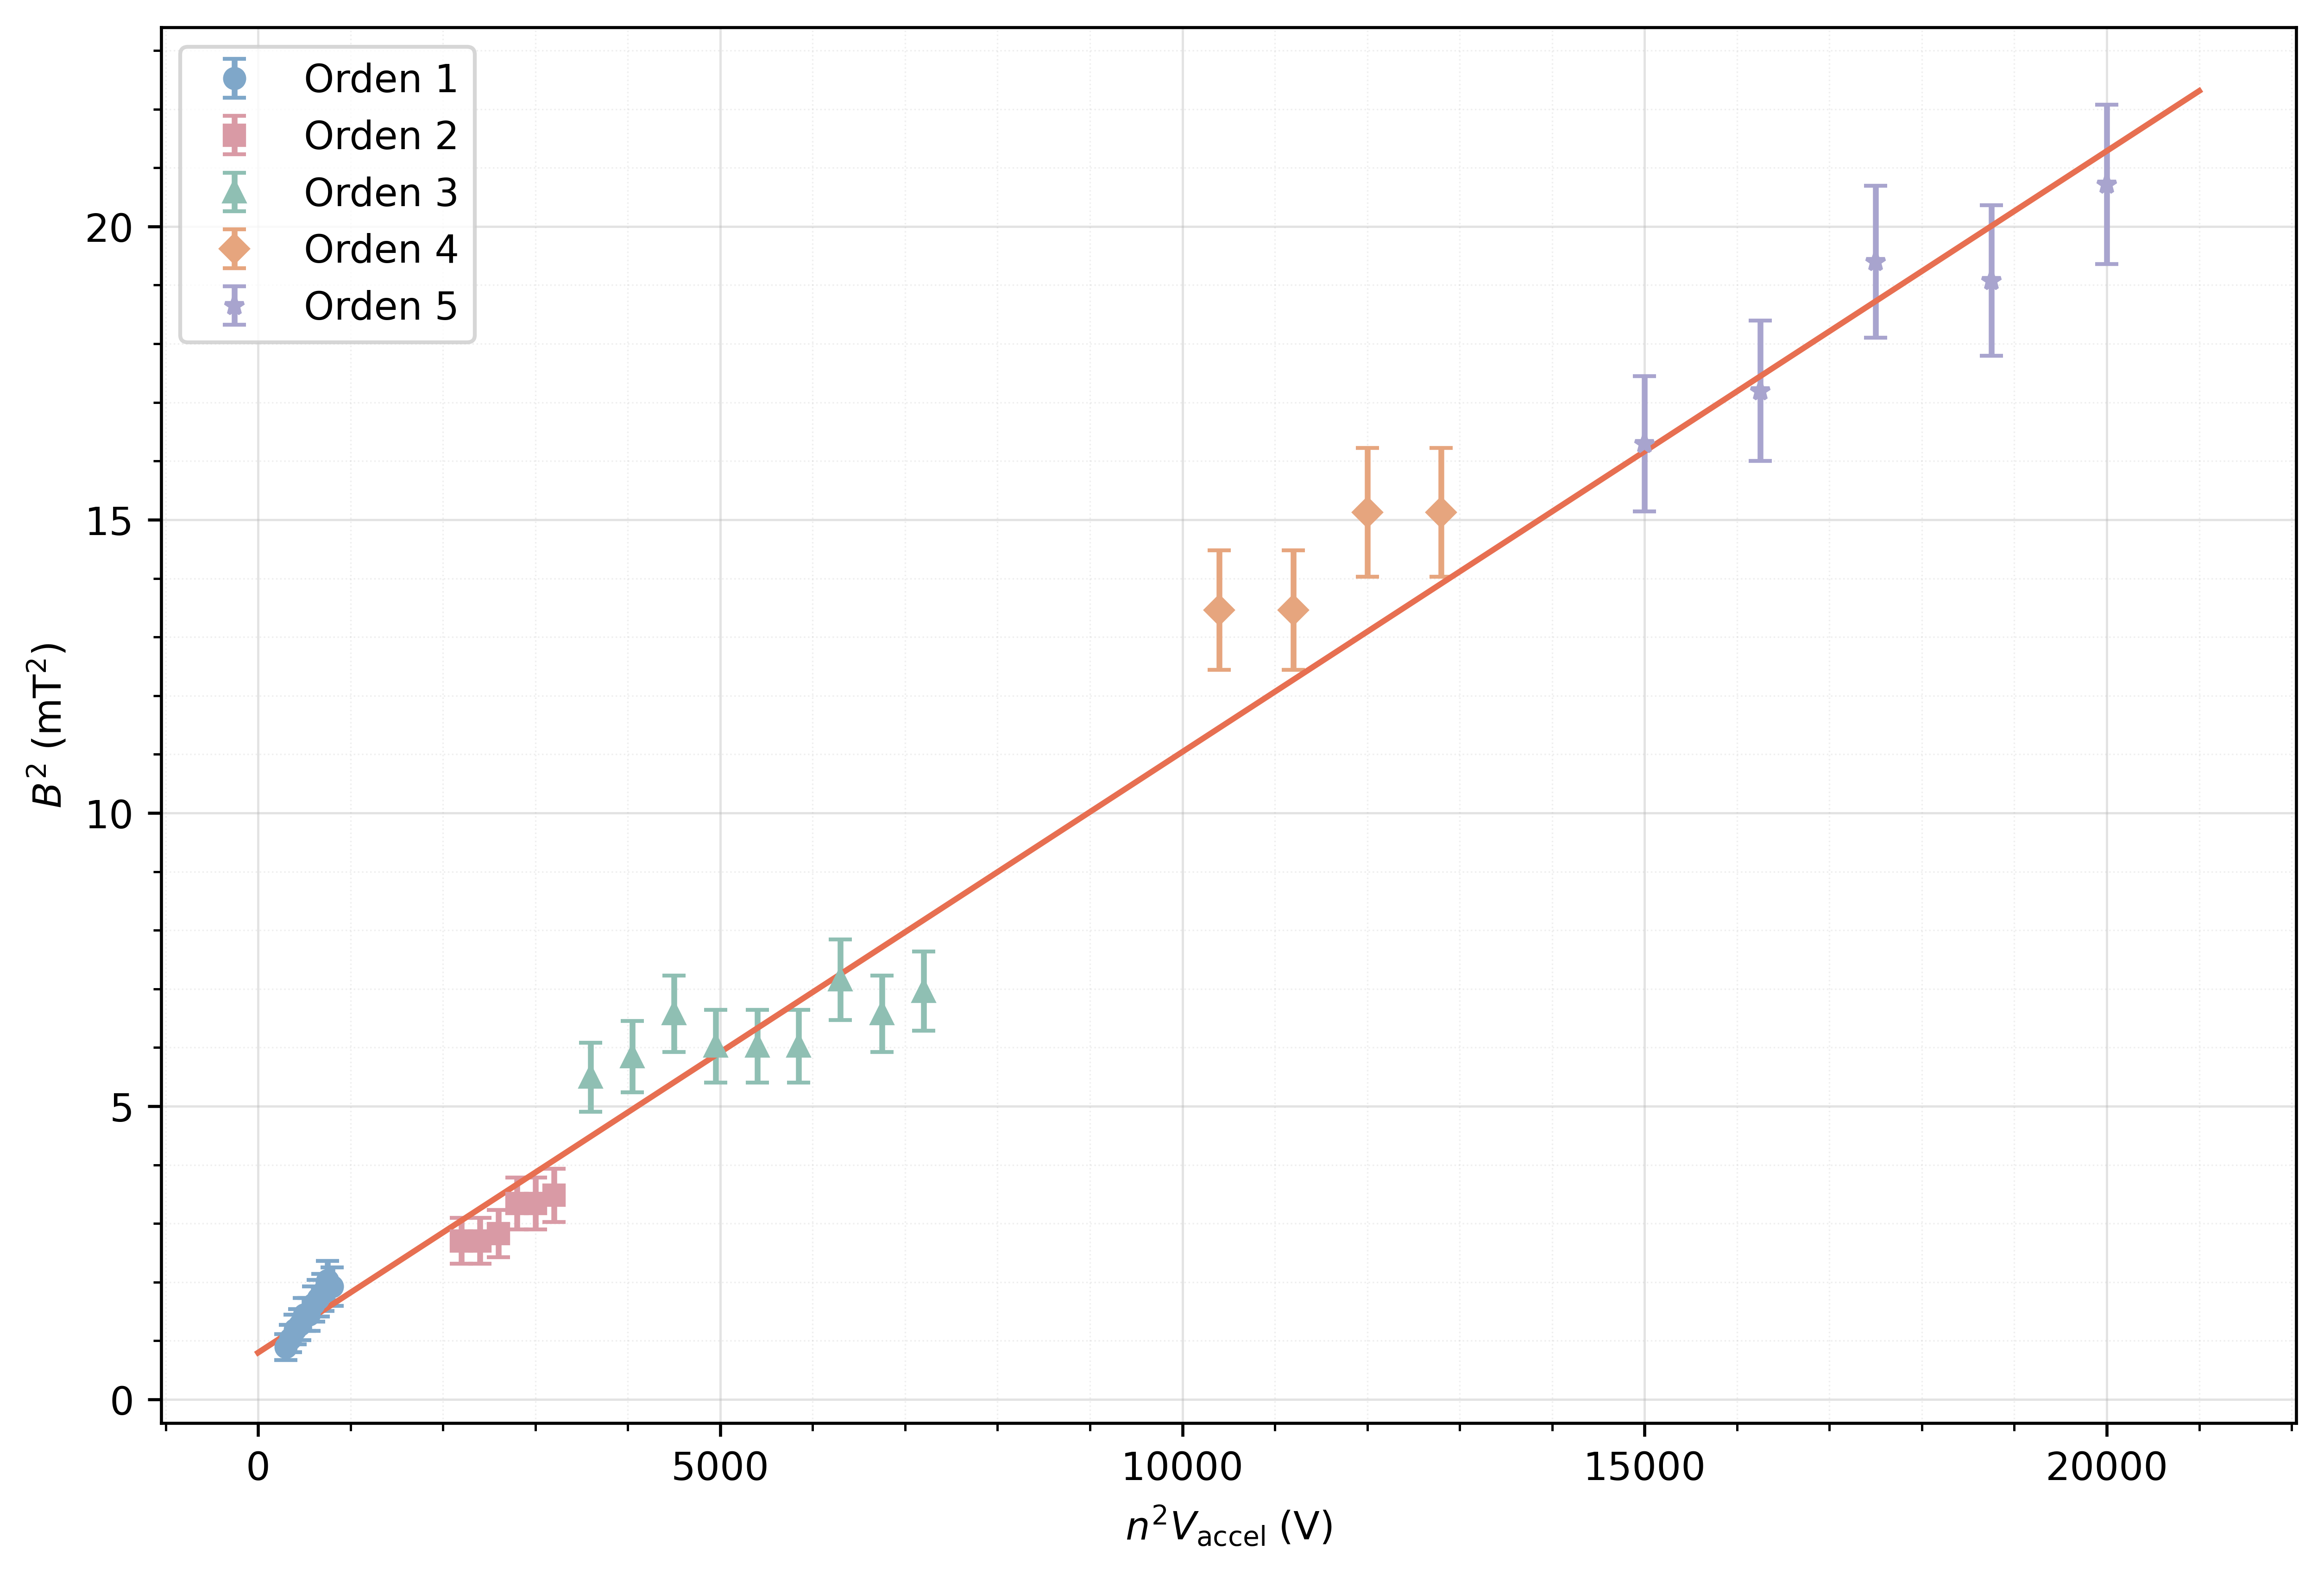
\includegraphics[width=\columnwidth]{Images/Ajuste_Bn2V.png}
    \caption{Valores de campo magnético $B$ que minimizan el área relativa en función de la tensión de aceleración $V,$ normalizados por $n^2,$ junto a su ajuste}
    \label{fig:minimos_normalizados}
\end{figure}

A partir de la pendiente del ajuste y la Ecuación ECUACION QUE HAY QUE PONER, se determinó que la relación
carga-masa del electrón es $e/m=\left( 6,7 \pm 0,4 \right)\times 10^{11}\,\unit{\coulomb\per\kilogram},$ valor lejano al aceptado de $1,75882000838(55)\times 10^{11}\,\unit{\coulomb\per\kilogram}$\cite{nist_em}.

Como en la Figura \ref{fig:minimos_normalizados} se observa que la pendiente de los valores para el primer orden es mayor (y por lo tanto una menor $e/m$), se
hizo un ajuste sobre esos datos únicamente para ver si estos eran más consistentes, pero el valor obtenido fue de $e/m=\left( 3,1 \pm 0,2 \right)\times 10^{11}\,\unit{\coulomb\per\kilogram},$ valor todavía
lejano del aceptado, aunque mejor que el obtenido anteriormente.

\section{Discusión}
Como se mostró, los resultados son inconsistentes con el valor aceptado. Esto se debe a distintos problemas
que surgieron a lo largo del experimento. En primer lugar la calibración del campo magnético.
Algo que sucedió es que una vez calibrado el campo magnético, al volver a medir el campo otro día bajo
las mismas condiciones de corriente $I$ y resistencias de los reóstatos, el valor cambiaba. En un primer
lugar se atribuyó esto a algún material ferromagnético cercano, pero al medir el campo magnético sin corriente se vió
que el valor del campo era únicamente el terrestre, por lo que se descartó esta hipótesis. Luego se atribuyó a la temperatura,
pero los campos fueron medidos con un ventilador prendido para que no se sobrecalienten las bobinas, por lo que esto fue descartado también.
Nuestra hipótesis final es que haya cambiado el valor de resistencia de alguna de las bobinas, lo que haría que cambie el
valor de $I$ y por tanto de $B.$

Esto hizo, entre otras cosas, que no sepamos realmente qué tan homogéneo es el campo magnético ni tampoco su valor, sino que se supuso que no cambió
desde la última calibración, lo que no es necesariamente cierto. Esto explica por qué la curva de área relativa de impacto en función
de la tensión de alimentación en la Figura \ref{fig:area_vs_V} no sigue dicha forma para algunos valores de $V,$ ya que para que esto suceda debería haber un
campo constante $B.$

Por último, debido a que la fuente de corriente utilizada inicialmente no suministraba un valor de $I$ confiable,
se tuvo que usar otra fuente de alimentación, la cual era comandada analógicamente por otra fuente, de modo que se introdujo un error adicional al tener que
realizar otra calibración para relacionar el valor de la tensión de alimentación con $B.$

Todos estos fueron limitantes para el experimento planteado donde se buscó recrear el Método de Busch para la determinación de la relación e/m.
Sin embargo, a pesar de aquellos, se alcanzó un resultado del mismo orden de magnitud que el valor tabulado, $\left( 6,7 \pm 0,4 \right)\times 10^{11}\,\unit{\coulomb\per\kilogram}$ (o $\left( 3,1 \pm 0,2 \right)\times 10^{11}\,\unit{\coulomb\per\kilogram}$ en el caso del primer orden de mínimos), 
contra $1,75882000838(55)\times 10^{11}\,\unit{\coulomb\per\kilogram}$. Se pudo, entonces, conocer la relación entre la carga y la masa del electrón en su magnitud,
mas no puede aún afirmarse que el experimento, tal como aquí fue planteado, sea satisfactorio para la obtención de una relación consistente con la tabulada.

\section{Conclusiones}
Se logró medir la relación carga-masa del electrón, resultando en $e/m=\left( 6,7 \pm 0,4 \right)\times 10^{11}\,\unit{\coulomb\per\kilogram},$ lo que no es consistente con el valor aceptado.
Esto se debe probablemente a lo anteriormente discutido.

En definitiva, el experimento se vio afectado por distintos problemas que hicieron que los resultados no sean consistentes con el valor aceptado, por lo
que debería ser repetido, teniendo en cuenta los problemas mencionados anteriormente, para obtener mejores resultados, principalmente
lograr una buena calibración del campo magnético, ya que esto es una suposición fundamental para el análisis de los resultados.

\section*{Referencias}
\renewcommand{\refname}{}

\bibliographystyle{ieeetr}
\bibliography{sources.bib}

\clearpage
% ================== ANEXO: Propagación de errores ==================
\appendix
\section{Anexo A: Calibración del campo magnético}
\label{anexo:a}

Al comenzar la calibración, se comenzó con el valor de resistencias dadas por Pandiani y Sarasola \cite{Pandiani}. A partir
de dichos valores se midió el campo magnético a lo largo del cilindro. Las zonas con un bajo $|\mathbf{B}|$ indicaban que se necesitaba más corriente
por lo que se disminuían las resistencias de los reóstatos de las bobinas de dicha zona. De manera análoga, si el campo magnético era demasiado alto, se aumentaban las resistencias.
Este proceso se repitió reiteradas veces hasta alcanzar un campo lo suficientemente homogéneo. Esto se alcanzó para los valores de resistencia presentados en la Tabla \ref{tab:resistencias}.

\begin{table}[h]
    \centering
    \begin{tabular}{cS}
        \toprule
        Reóstato & {Resistencia (\unit{\ohm})} \\
        \hline
        A1 & 32,3 \pm 0,1 \\
        A2 & 60,0 \pm 0,1\\
        A3 & 22,4 \pm 0,1 \\
        B1 & 3,1 \pm 0,1 \\
        B2 & 4,5 \pm 0,1 \\
        \bottomrule
    \end{tabular}
    \caption{Resistencias finales de los reóstatos para cada bobina.}
    \label{tab:resistencias}
\end{table}

Se hicieron barridos para distintos valores de corriente y se midió el campo magnético en distintos puntos del cilindro.
Con los datos se cada corriente, se tomó un valor promedio de $B$ a lo largo del cilindro y se ajustó dicho valor en función de la corriente. El resultado se muestra en la Figura \ref{fig:calibracion}.

\begin{figure}[!h]
    \centering
    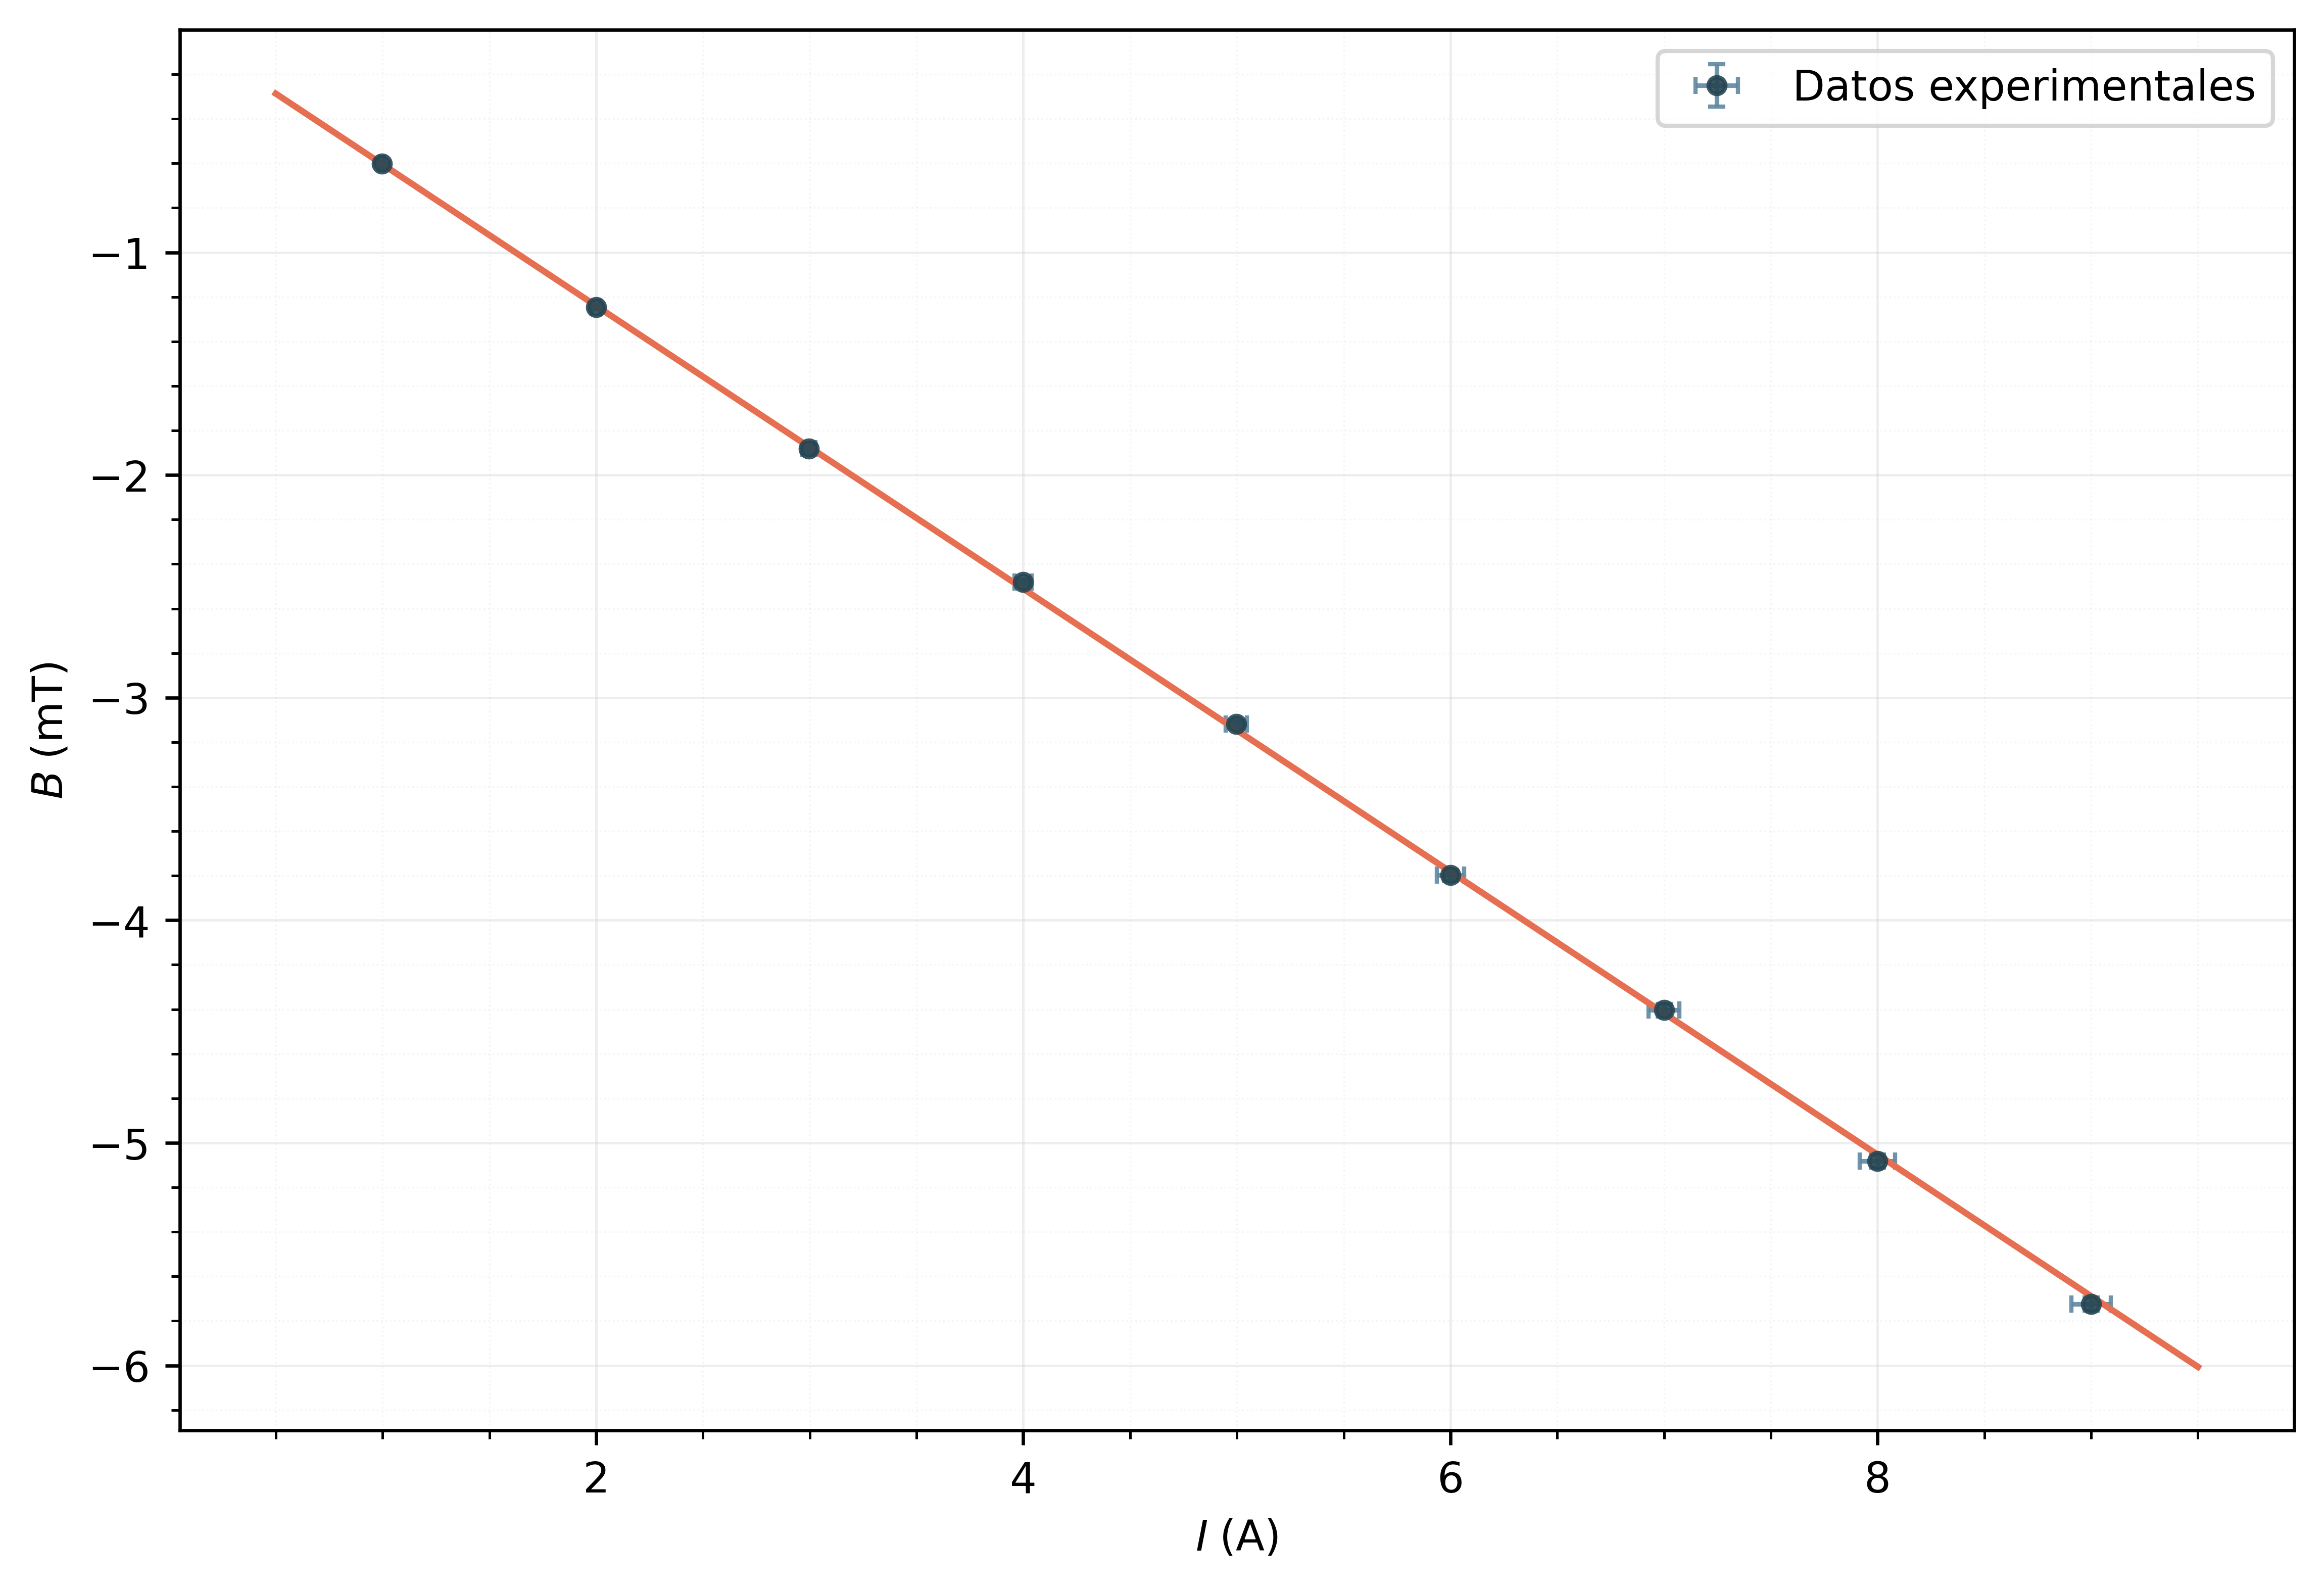
\includegraphics[width=0.45\textwidth]{Images/ajusteBI.png}
    \caption{Curva de calibración del campo magnético en función de la corriente.}
    \label{fig:calibracion}
\end{figure}

\section{Anexo B: Calibración de la fuente de corriente e identificación de mínimos}
\label{anexo:b}

Debido a que la fuente usada inicialmente para alimentar las bobinas, la GW Instek PSH-3620A, no entregaba la corriente que 
decía entregar, se optó por el uso de una fuente HP 6268B, la cual se comandaba analógicamente mediante una GW Instek GPS-4303S,
ya que esta necesita ser suministrada con tensión para entregar una corriente proporcional. Por esto se hizo una calibración de la fuente HP 6268B, para saber así que
corriente circula por el sistema en función de la tensión suministrada por la GPS-4303S. La curva de ajuste se muestra en la Figura \ref{fig: ajuste_fuente}

\begin{figure}[!h]
    \centering
    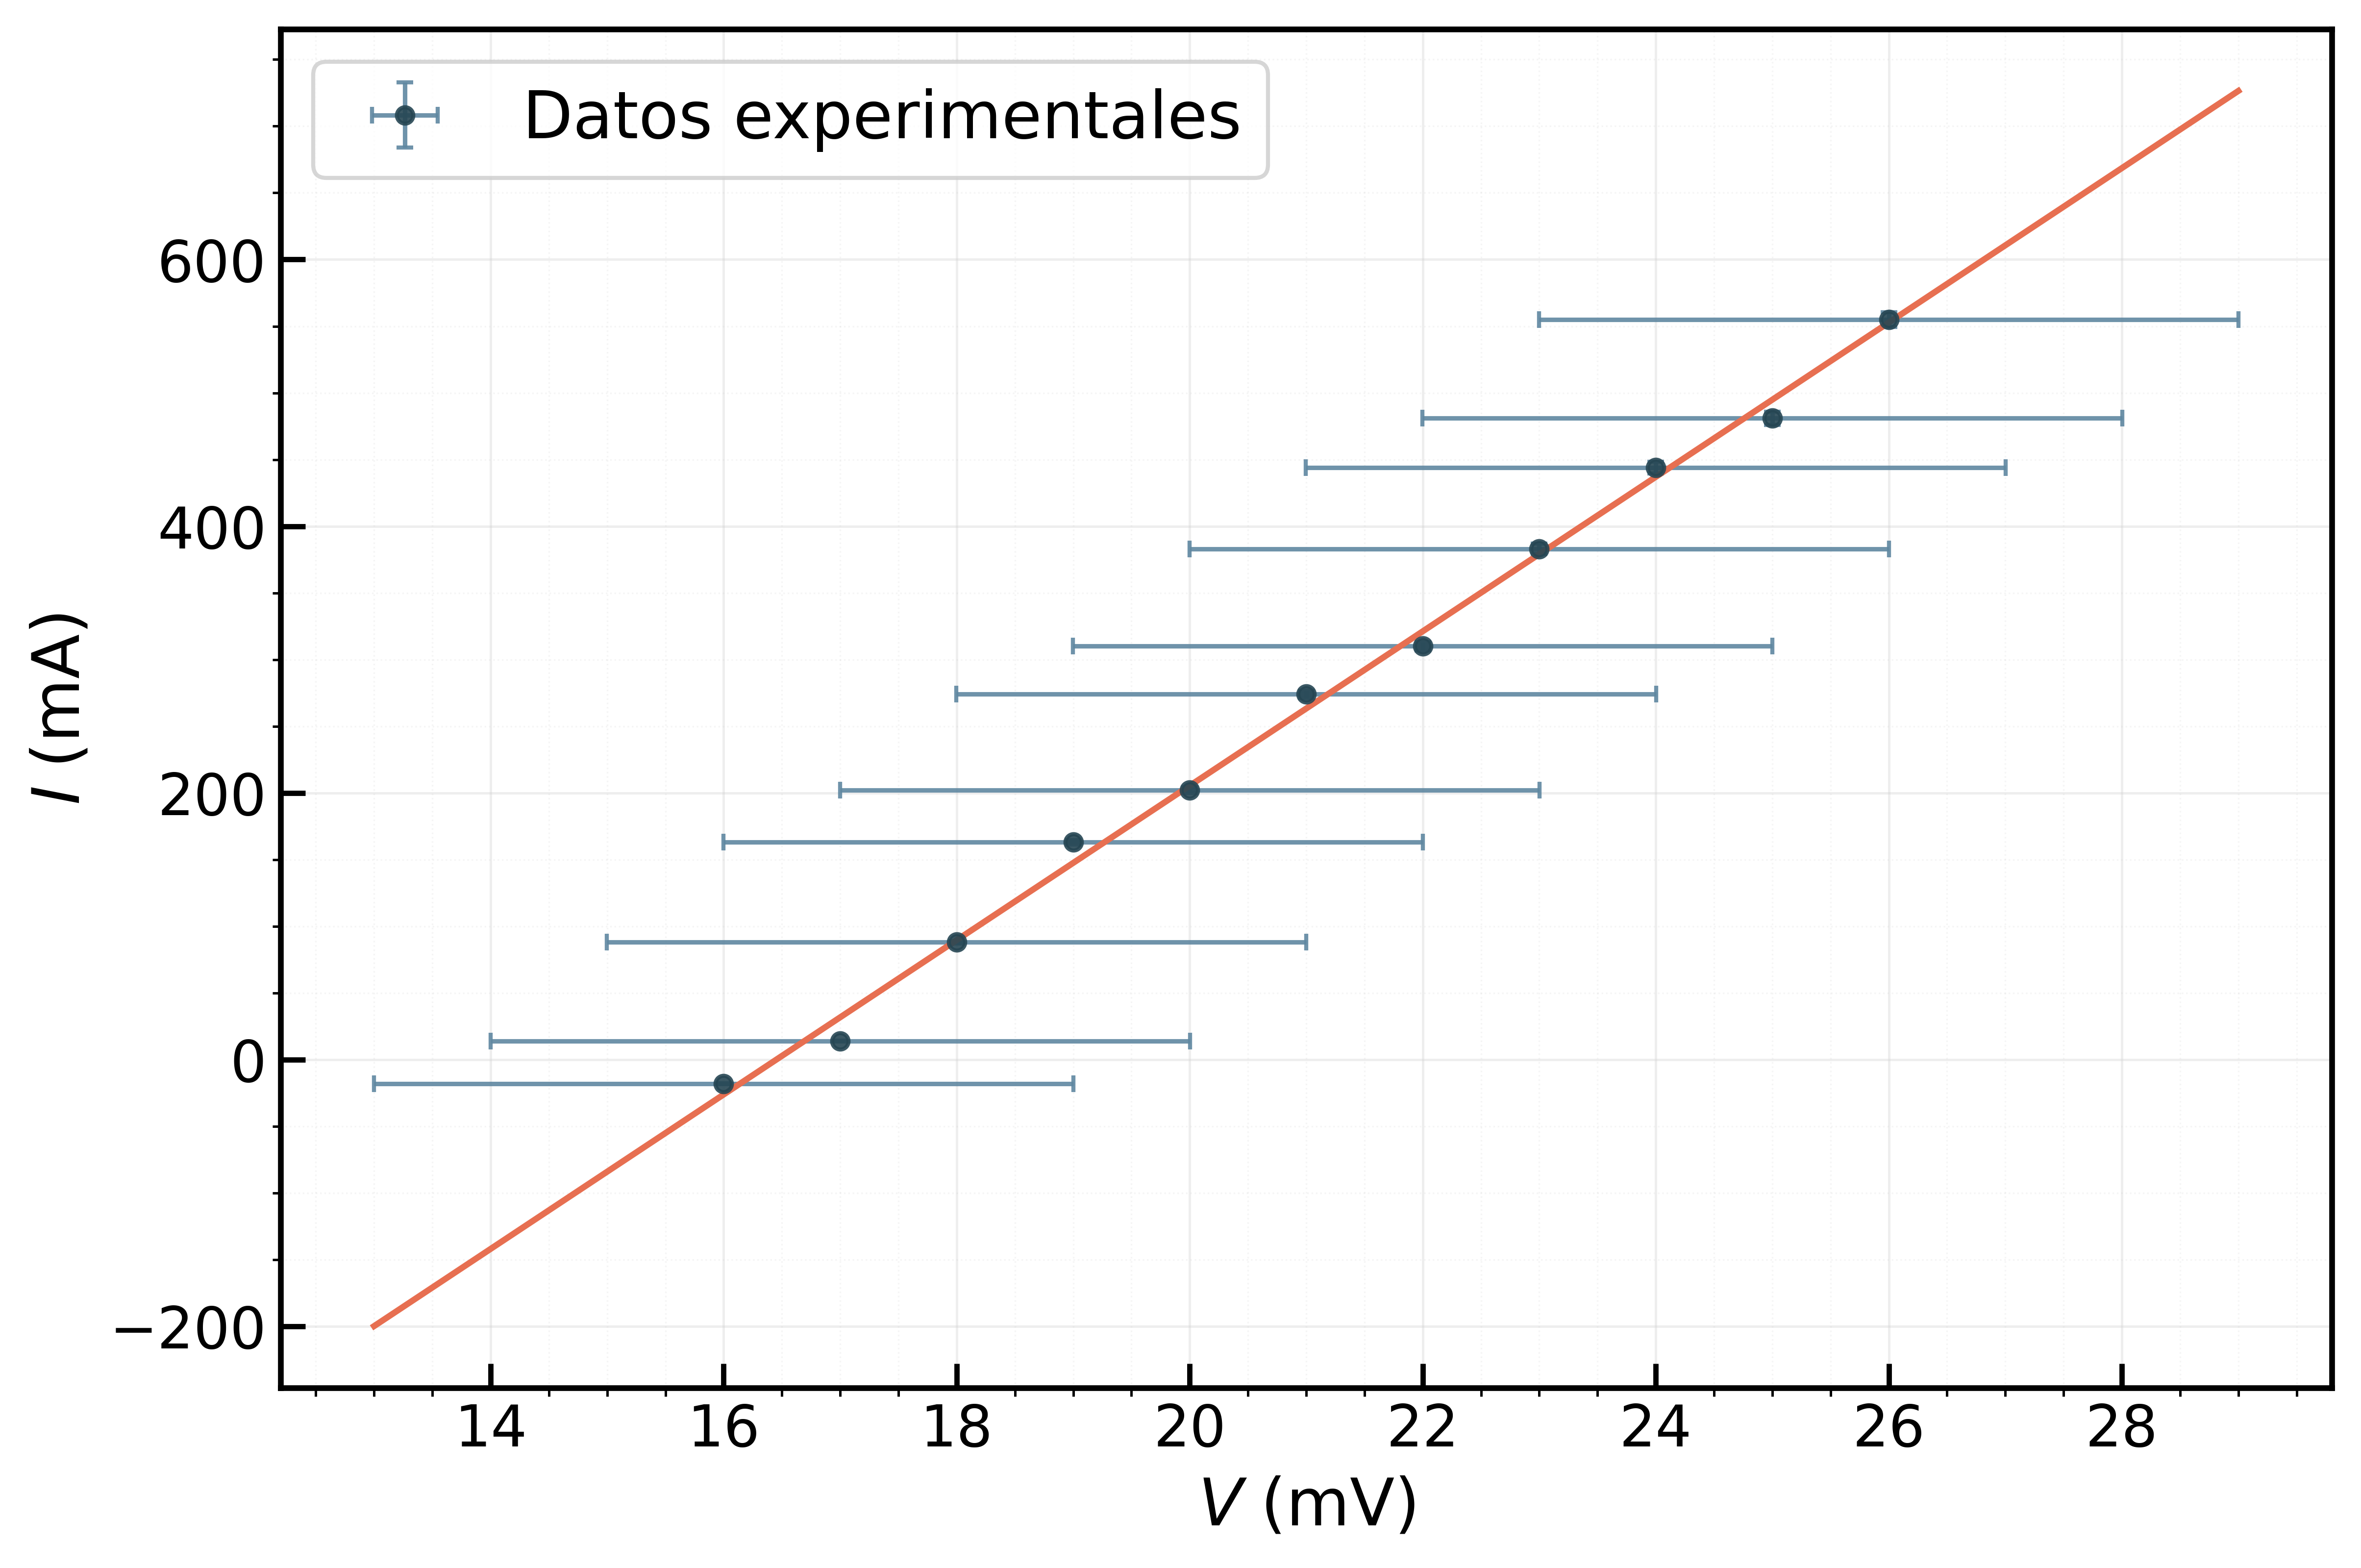
\includegraphics[width=0.49\textwidth]{Images/AjusteVI.png}
    \caption{Curva de calibración de la corriente entregada por la fuente HP 6268B en función de la tensión suministrada por la fuente GW Instek GPS-4303S.}
    \label{fig: ajuste_fuente}
\end{figure}

Luego para detectar los mínimos se hizo uso de un script de Python para comandar la cámara, tomar imágenes de la zona de impacto de los electrones,
calcular el área de impacto relativa, aumentar en $\SI{1}{\milli\volt}$ la tensión suministrada por la GPS-4303S, y repetir el proceso, almacenando los valores de tensión, área relativa y tensión de aceleración
utilizada en dicho barrido.

Para el cálculo del área de impacto relativa se toman los píxeles registrados y su intensidad. Si dicha intensidad es mayor a un umbral dado, llamado \textit{threshold}, se considerá que en ese píxel impactaron electrones.
Luego se calcula el área de impacto relativa como el número de píxeles que superan dicho umbral dividido por el número total de píxeles. Esto se hace para varios frames, a modo de tener un valor promedio de área relativa para cada tensión suministrada por la GPS-4303S.


\end{document}
